\documentclass[a4paper,10pt,oneside]{book}

% packages 
\usepackage{arsclassica}    % fancy layout
\usepackage[english]{babel}\addto{\captionsenglish}{\renewcommand{\bibname}{References}}
\usepackage{caption}         % figure captions
\usepackage[square,numbers,super,sort&compress]{natbib}  % bibliography style
\usepackage[cc]{titlepic}    % enable logo on title page
\usepackage{graphicx}       % logo related
\usepackage{float} 

\usepackage{standalone}

% don't hang captions
\captionsetup{format=plain}

% bibliography
\bibliographystyle{../thesis}

% title setup
\title{ \vspace{3in} Unravelling higher order genome organisation {\small [working
    title]} \\ \vspace{2em} {\large {\bf Introduction}} }
\author{Benjamin L. Moore}
\titlepic{\vspace{2.2in} 
\includegraphics[width=\textwidth]{/Users/benmoore/hvl/1yrReport/figs/igmm.png}}

\begin{document}

\maketitle

\chapter{Reanalysis of Hi-C datasets}

\section{Introduction}

Since the initial publication of the Hi-C technique in 2009,\cite{Lieberman2009} there has been rapid advancement of both the technique itself and the resolution at which interaction frequencies have been analysed. From the proof-of-concept analysis at 1 megabase (Mb) and 100 killable (kb) resolution,\cite{Lieberman2009} subsequent experiments achieved first 40 kb\cite{Dixon2012}, then 10 kb\cite{Jin2013} and most recently 1 kb\cite{Rao2014}, enabling bona fide fragment-level analysis for the first time.

% timeline: 
% Lieberman Aiden 2009       1 Mb (30 M reads)
% Dixon 2012                       40 kb (300 M reads)
% Jin 2013                        5-10 kb ()
% Rao 2014                           1 kb

Such rapid progression in the field has resulted in a wide variety of public Hi-C datasets being available, albeit with differing qualities. With proper correction and at a suitable resolution, these interaction frequencies can be compared and contrasted within and between species.

In this work I uniformly reprocessed publicly-available human Hi-C datasets, in order to address fundamental questions about the stability of higher order genome organisation within cell populations from the same species. Previously Hi-C studies have compared two samples per species, such as K562 against GM06990\cite{Lieberman2009} or IMR90 against GM12878.\cite{Dixon2012} Here I make use of three Hi-C datasets corresponding to extensively-studied human cell lines: K562, GM12878 and H1 hESC. Together these make up the "Tier 1" cell lines studied by the ENCODE consortium,\cite{Dunham2012} hence have huge amounts of matched ChIP-seq and histone modification data available. 

By combinatorial reanalysis of these cell-matched datasets, I can investigate the relationships between higher order chromatin structure and locus-level chromatin features.

% Table: description of cell lines

\section{Hi-C reprocessing}

Each Hi-C dataset used in this work was reprocessed using the same pipeline from raw sequencing reads. In each case, experiments used the same HindIII restriction enzyme.

% Pipeline:
% 1. iterative mapping
% 2. 

% figure showing contact maps, before and after (split cell type?)

\section{Compartment profiles}
% how well do compartments correlate

After uniformly reprocessing each Hi-C dataset and calling compartment eigenvector profiles (see \emph{Methods}), we can compare these between three human cell lines. Compartment profiles have a visibly high-correspondence (Fig. \ref{fig:wiggles}), despite the variable sources of both sample material and experimental data.

\begin{figure}
\begin{center}
\makebox[\textwidth][c]{ 
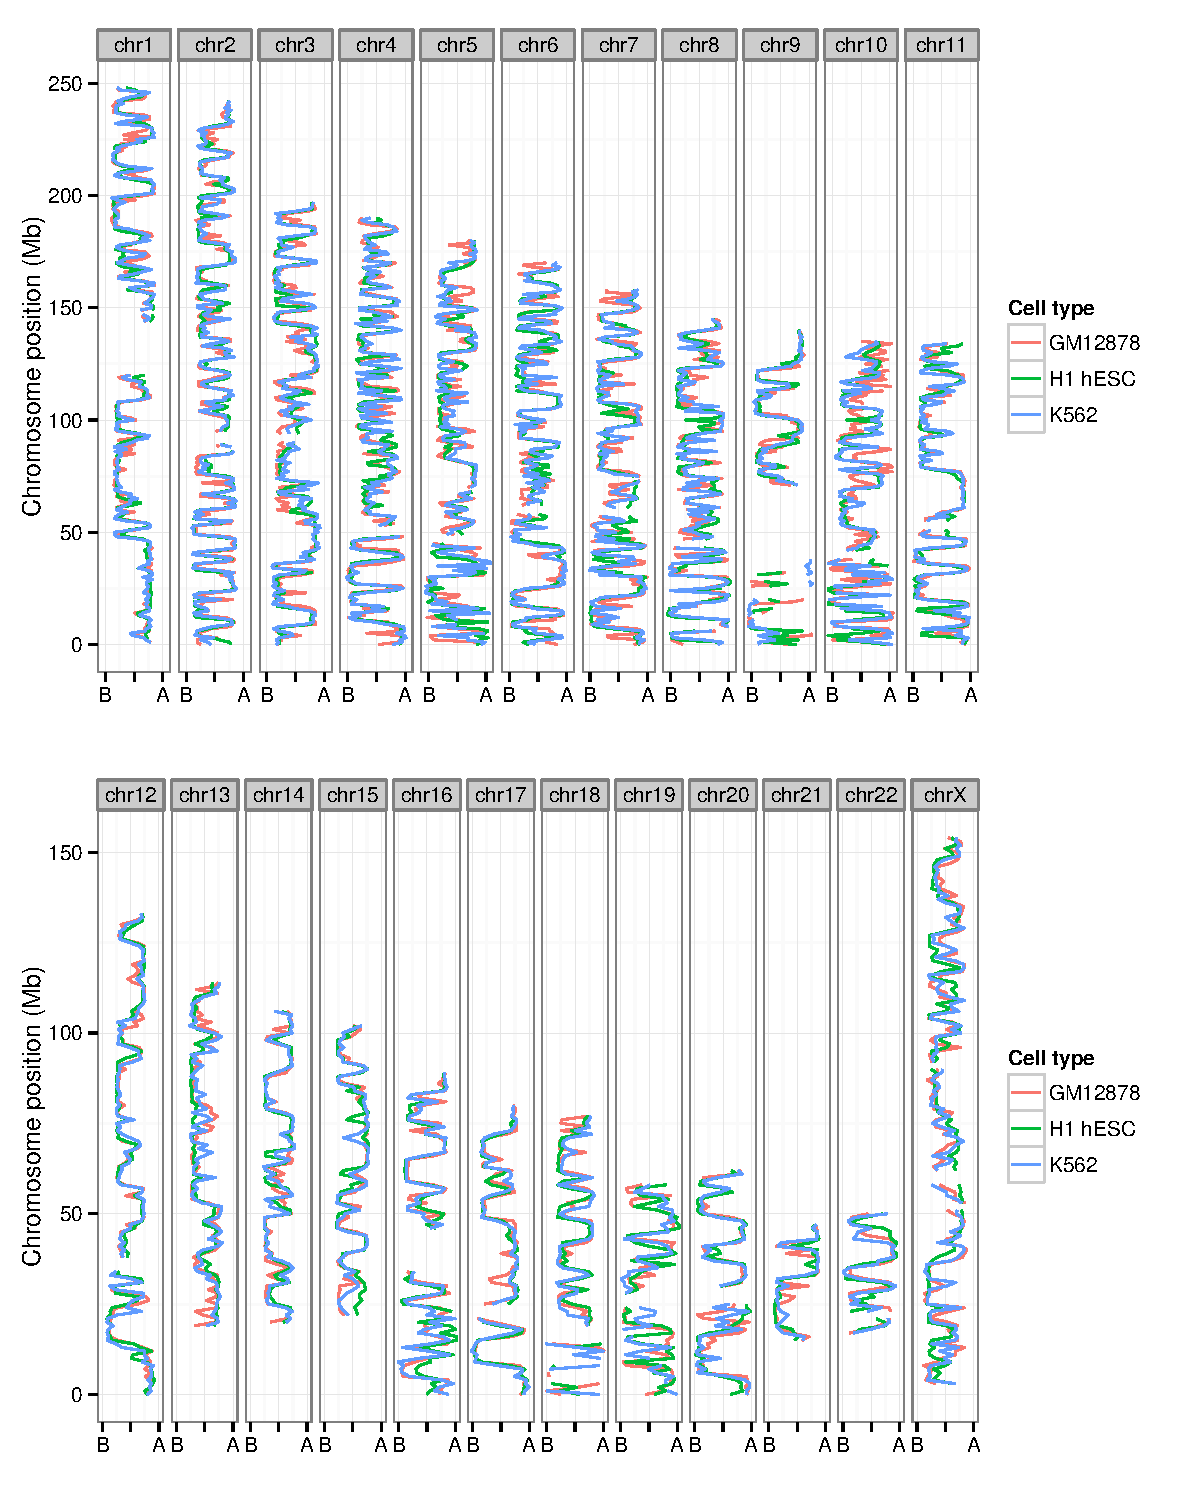
\includegraphics[width=1.2\textwidth]{figs/wiggles.pdf}
}
\captionsetup{width=\textwidth}
\caption{
{\bf Compartment profiles are observably well-correlated between human cell types and across all chromosomes.}
Caption
}\label{fig:wiggles}
\end{center}
\end{figure} 

This close correspondence also validates our approach of combining these different datasets, and suggests our uniform pipeline is successfully accounting for differences in sequencing depth and other batch effects. The precise correlations of these independent measures are in the interval $R = [.75, .8]$ (Fig. \ref{fig:compactor}; Pearson correlation coefficients, PCC).

\begin{figure}
\begin{center}
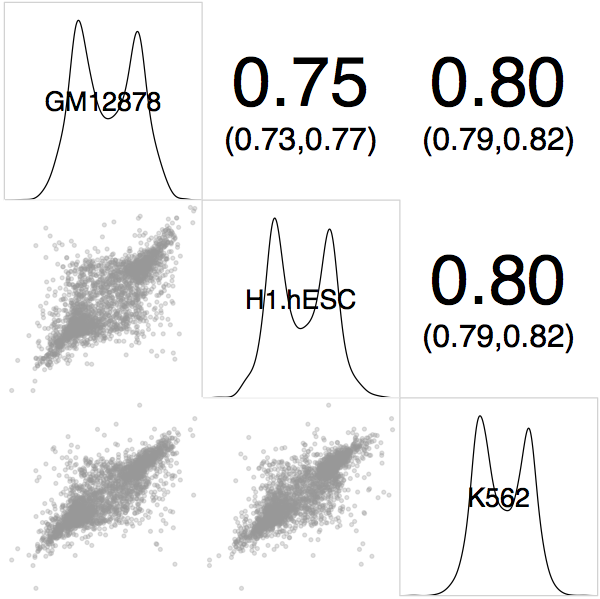
\includegraphics[width=.5\textwidth]{figs/compartment_corr.png}
\captionsetup{width=\textwidth}
\caption{
{\bf Compartment eigenvectors are well-correlated between human cell types}
Megabase resolution compartment eigenvector values are shown in a plot matrix. \emph{Upper triangle}: Pearson correlation coefficients between pairs, with $95\%$ confidence intervals; \emph{diagonal} Kernel density estimates of eigenvector values per cell type; \emph{lower triangle}: $x$-$y$ scatterplot of values.
}\label{fig:compcor}
\end{center}
\end{figure} 

\section{Domain calls}

\subsection{Compartments}

The continuous compartment eigenvector can be used as-is to classify A/B compartments, using positive and negative eigenvector values after first orientating the vector with respect to, for example, PolII Chip-seq data.\cite{Kalhor2012} However, given the definition of compartments as generally broad and alternating domains along a chromosome, often matching other large domains of Lamin association, an improved classification method might penalise the calls of short compartment calls, which may be the result of noise.

For this reason, instead of using raw eigenvector values we consider observed values as emissions from unobserved underlying states. This can be modelled through a Hidden Markov Model (HMM), whereby we first parameterise models of state and their transitions, then infer the most likely state sequence to have emitted our observed data. This unobserved two-state sequence is then used for compartment calls (see Methods \ref{sec:eigs}). 

In practice, this acts to de-noise our compartment calls. Where single sign-changes along the series would have resulted in a single-block compartment, these may now be modelled as noisy emissions from a single unobserved state. An examplar region is showing in Fig. \ref{fig:denoise}. This shows an approximately 50 Mb region from chromosome 8 with eigenvector data from the H1 hESC cell line. A simple thresholding method in this region calls a total of $12$ regions, whereas our HMM method finds only $6$ larger regions in the same window.The disparity is caused by very short and single-bin compartments being disfavoured by the HMM-based method (Fig. \ref{fig:denoise}). 

% figure showing raw eigs with hmm calls
\begin{figure}
\begin{center}
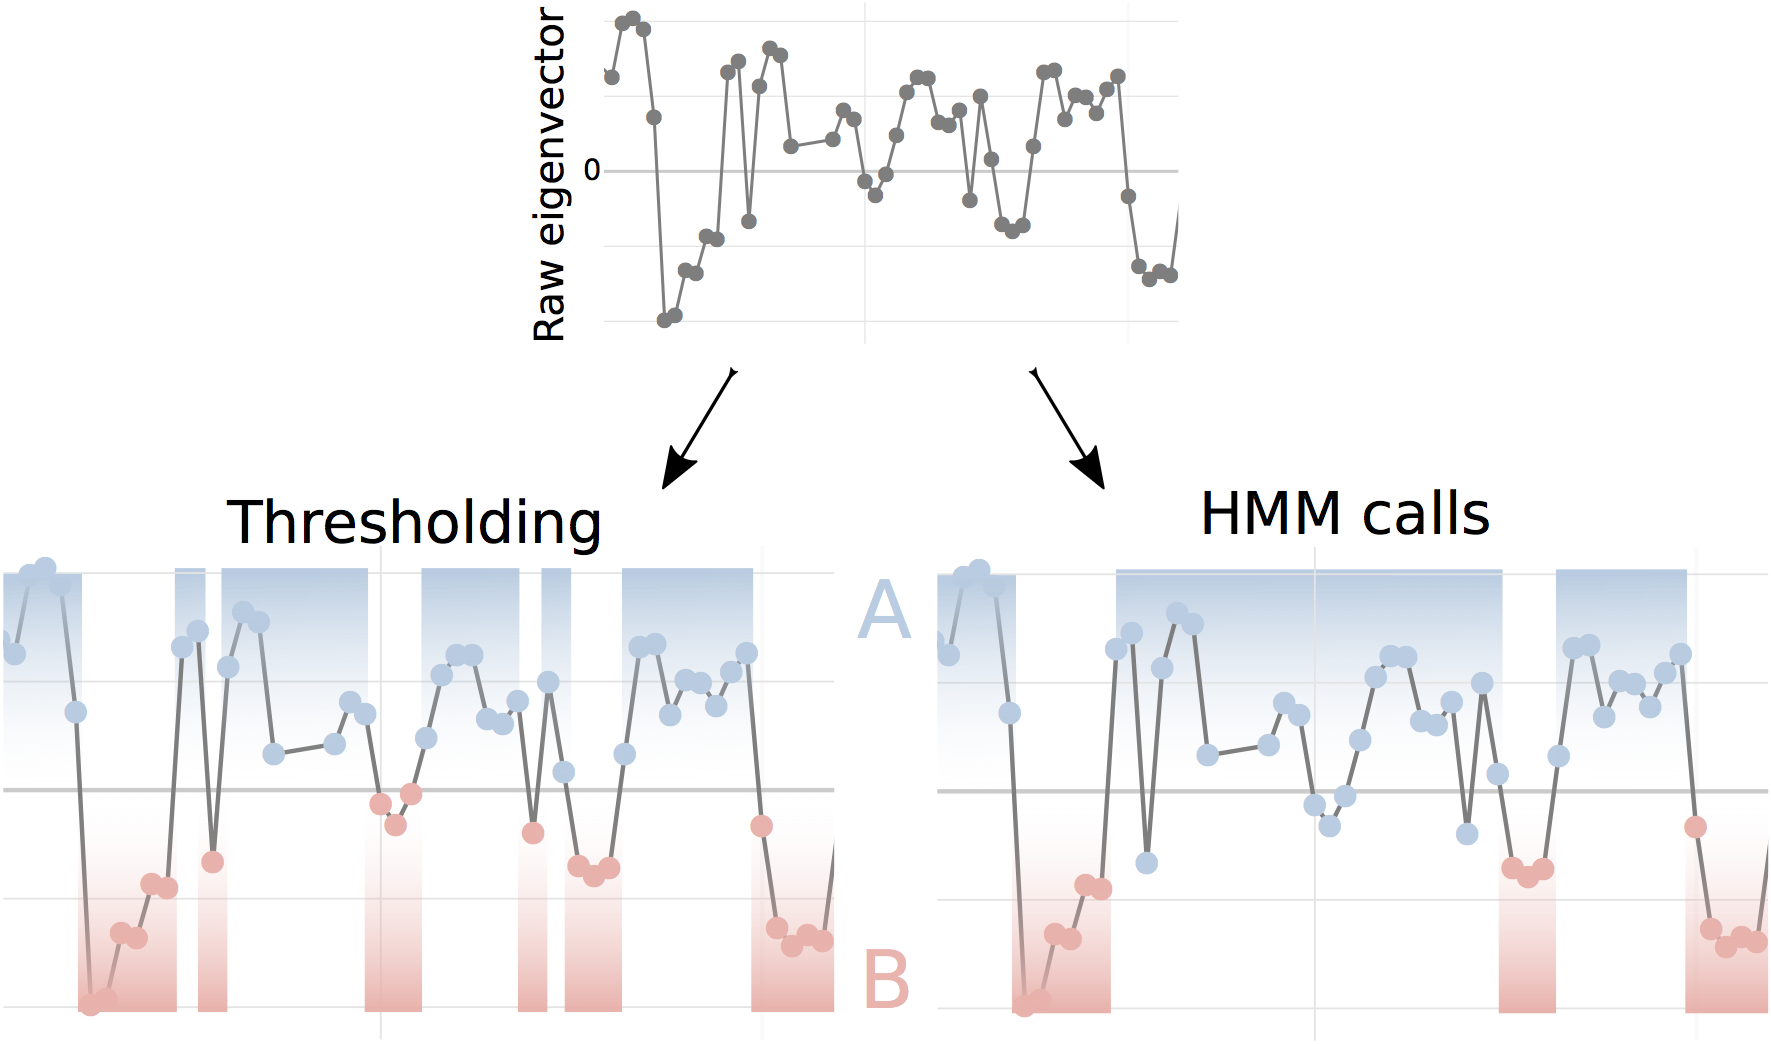
\includegraphics[width=.9\textwidth]{figs/hmm_calls.png}
\captionsetup{width=\textwidth}
\caption{ {\bf Compartment calls by simple thresholding method or context-aware HMMs.}
Chromosome compartments have previously been called through simple thresholding at $0$,\cite{Lieberman2009} in this work we also use an HMM-based method to call unobserved states that have emitted our noisy observed values (\emph{right}).
}\label{fig:denoise}
\end{center}
\end{figure} 


% figure showing size distributions of Hi-C domains


\subsection{TADs}

\begin{figure}
\begin{center} 
\makebox[\textwidth][c]{ 
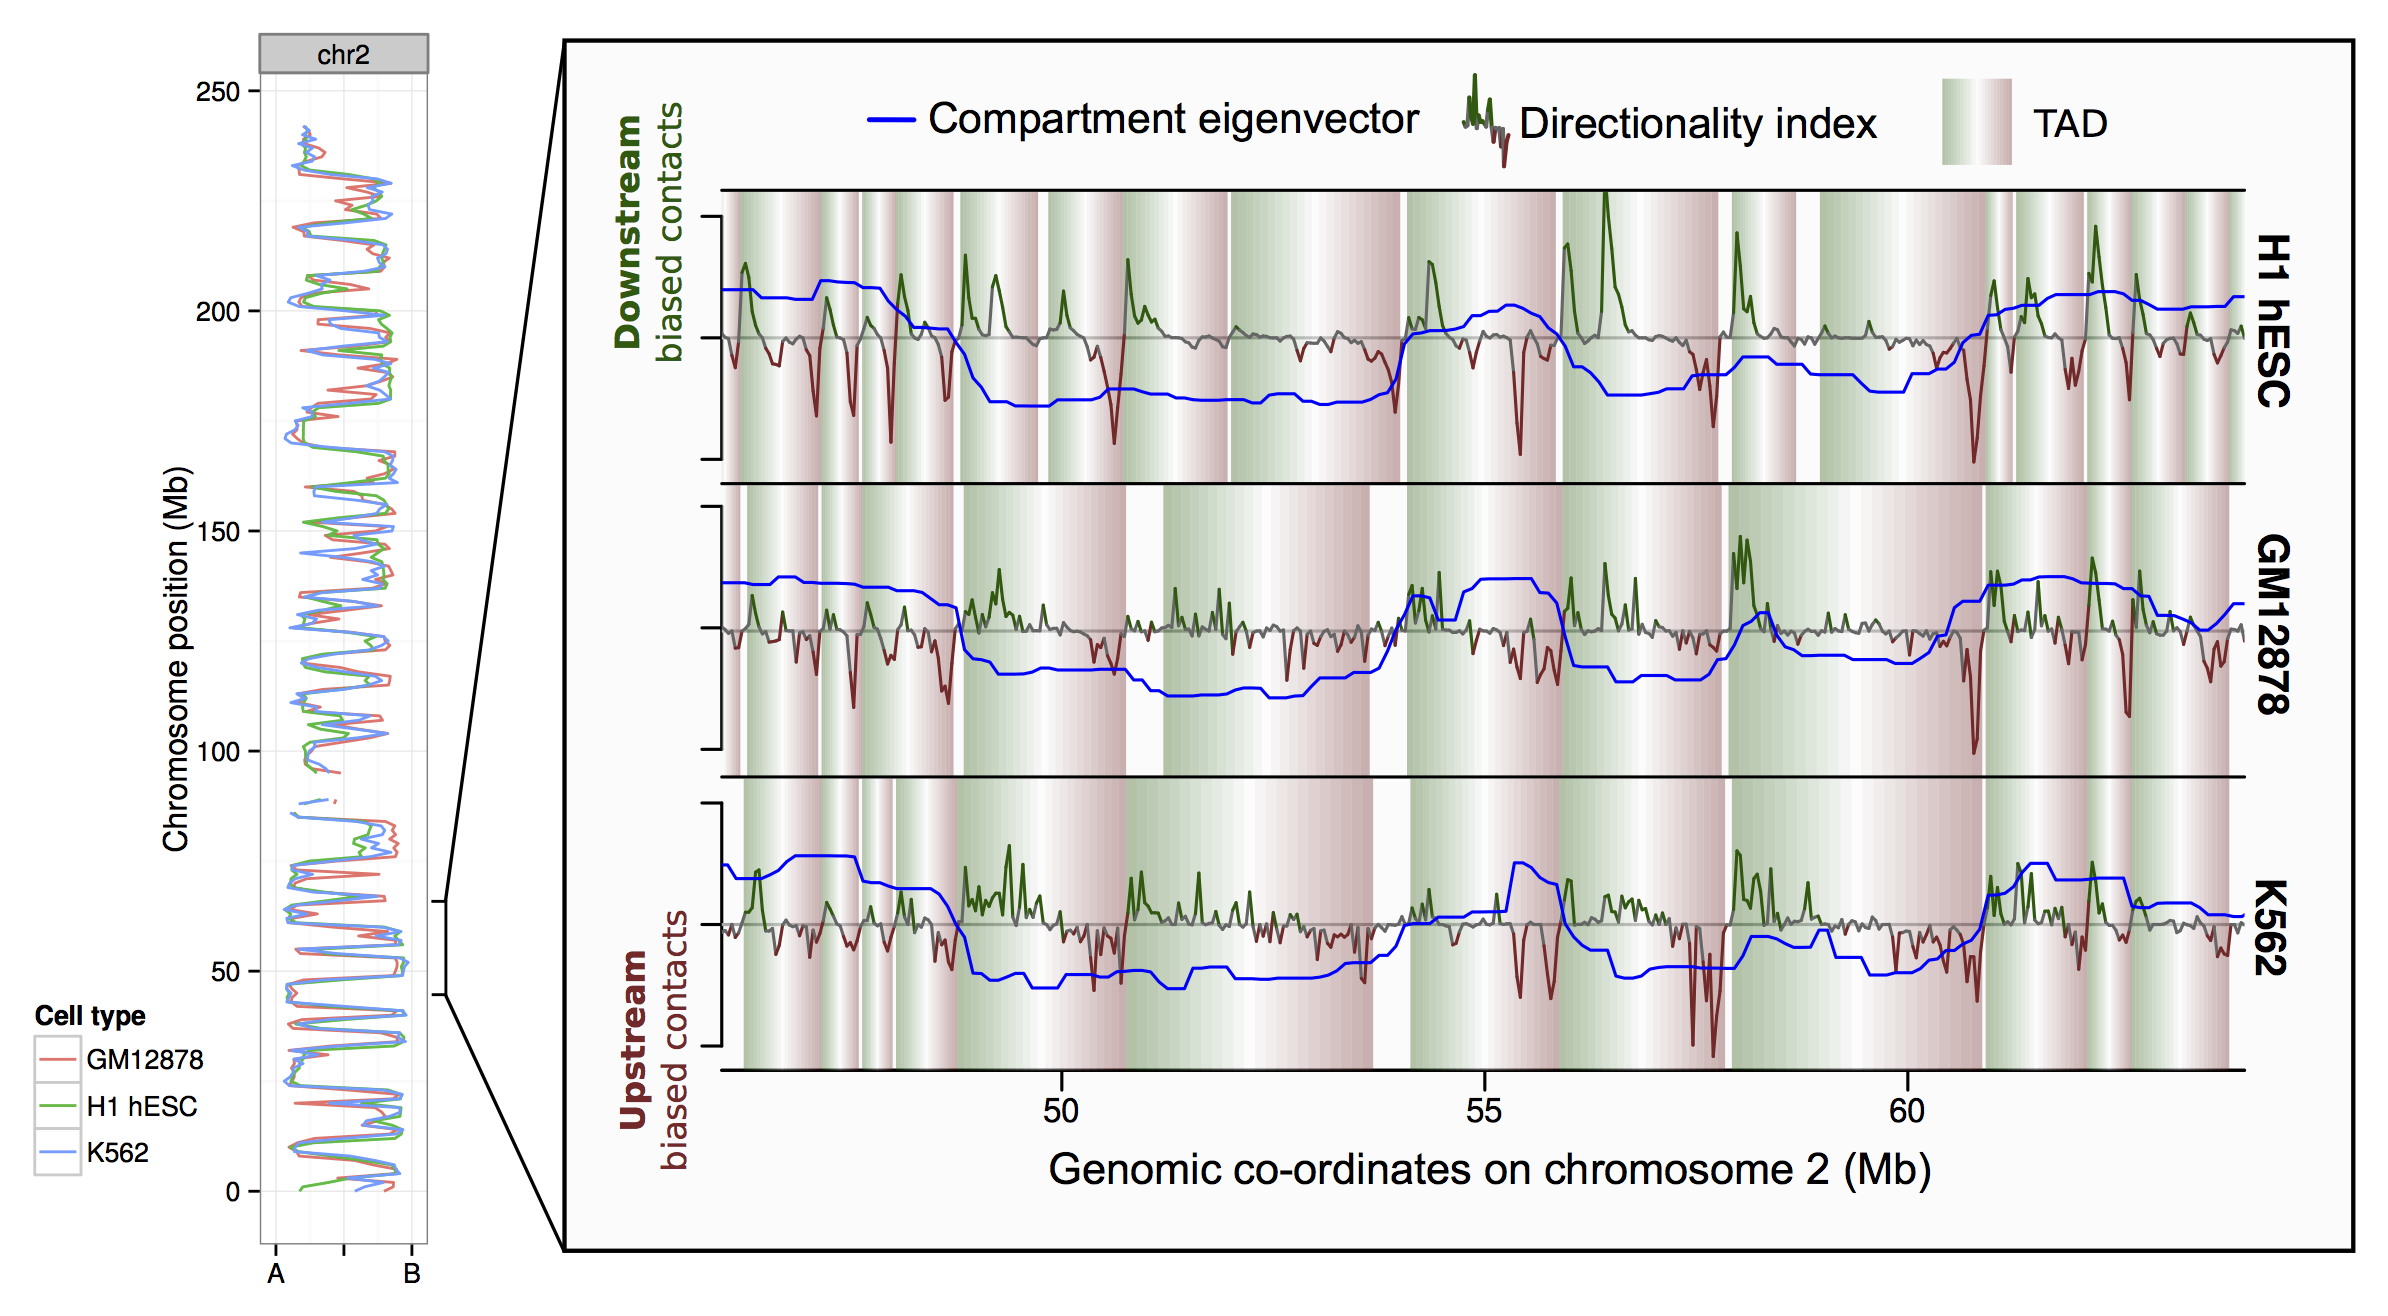
\includegraphics[width=1.2\textwidth]{figs/blowout.png}
}
\captionsetup{width=\textwidth} 
\caption{ {\bf Regions of variable structure alter their long-range contacts. }
The eigenvector compartment profile is shown for chromosome 2 for three human cell types (\emph{left}).  At higher resolution, the zoomed region illustrates conservation of topological domains (TADs) over 20 Mb of the same chromosome.
}\label{fig:blowout}
\end{center} 
\end{figure} 


\section{Variable regions}
% investigate those regions which are "flipped"

Despite the vast majority of the genome being in matched chromatin compartments, there are also regions of disagreement. Reasons for observable differences include technical errors and bias, but also more interesting functional explanations, where cell-type specific activation or repression is reflected in changes in higher order structure.

To conservatively call regions of variable structure (RVS), we used HMM-called compartment states and selected those which were either: i) open in one cell type and closed in both others or ii) closed in one cell type and open in both others. This left sets of RVS which could be considered as "flipped open" or "flipped closed" in a given cell type.

\begin{figure}
\begin{center} 
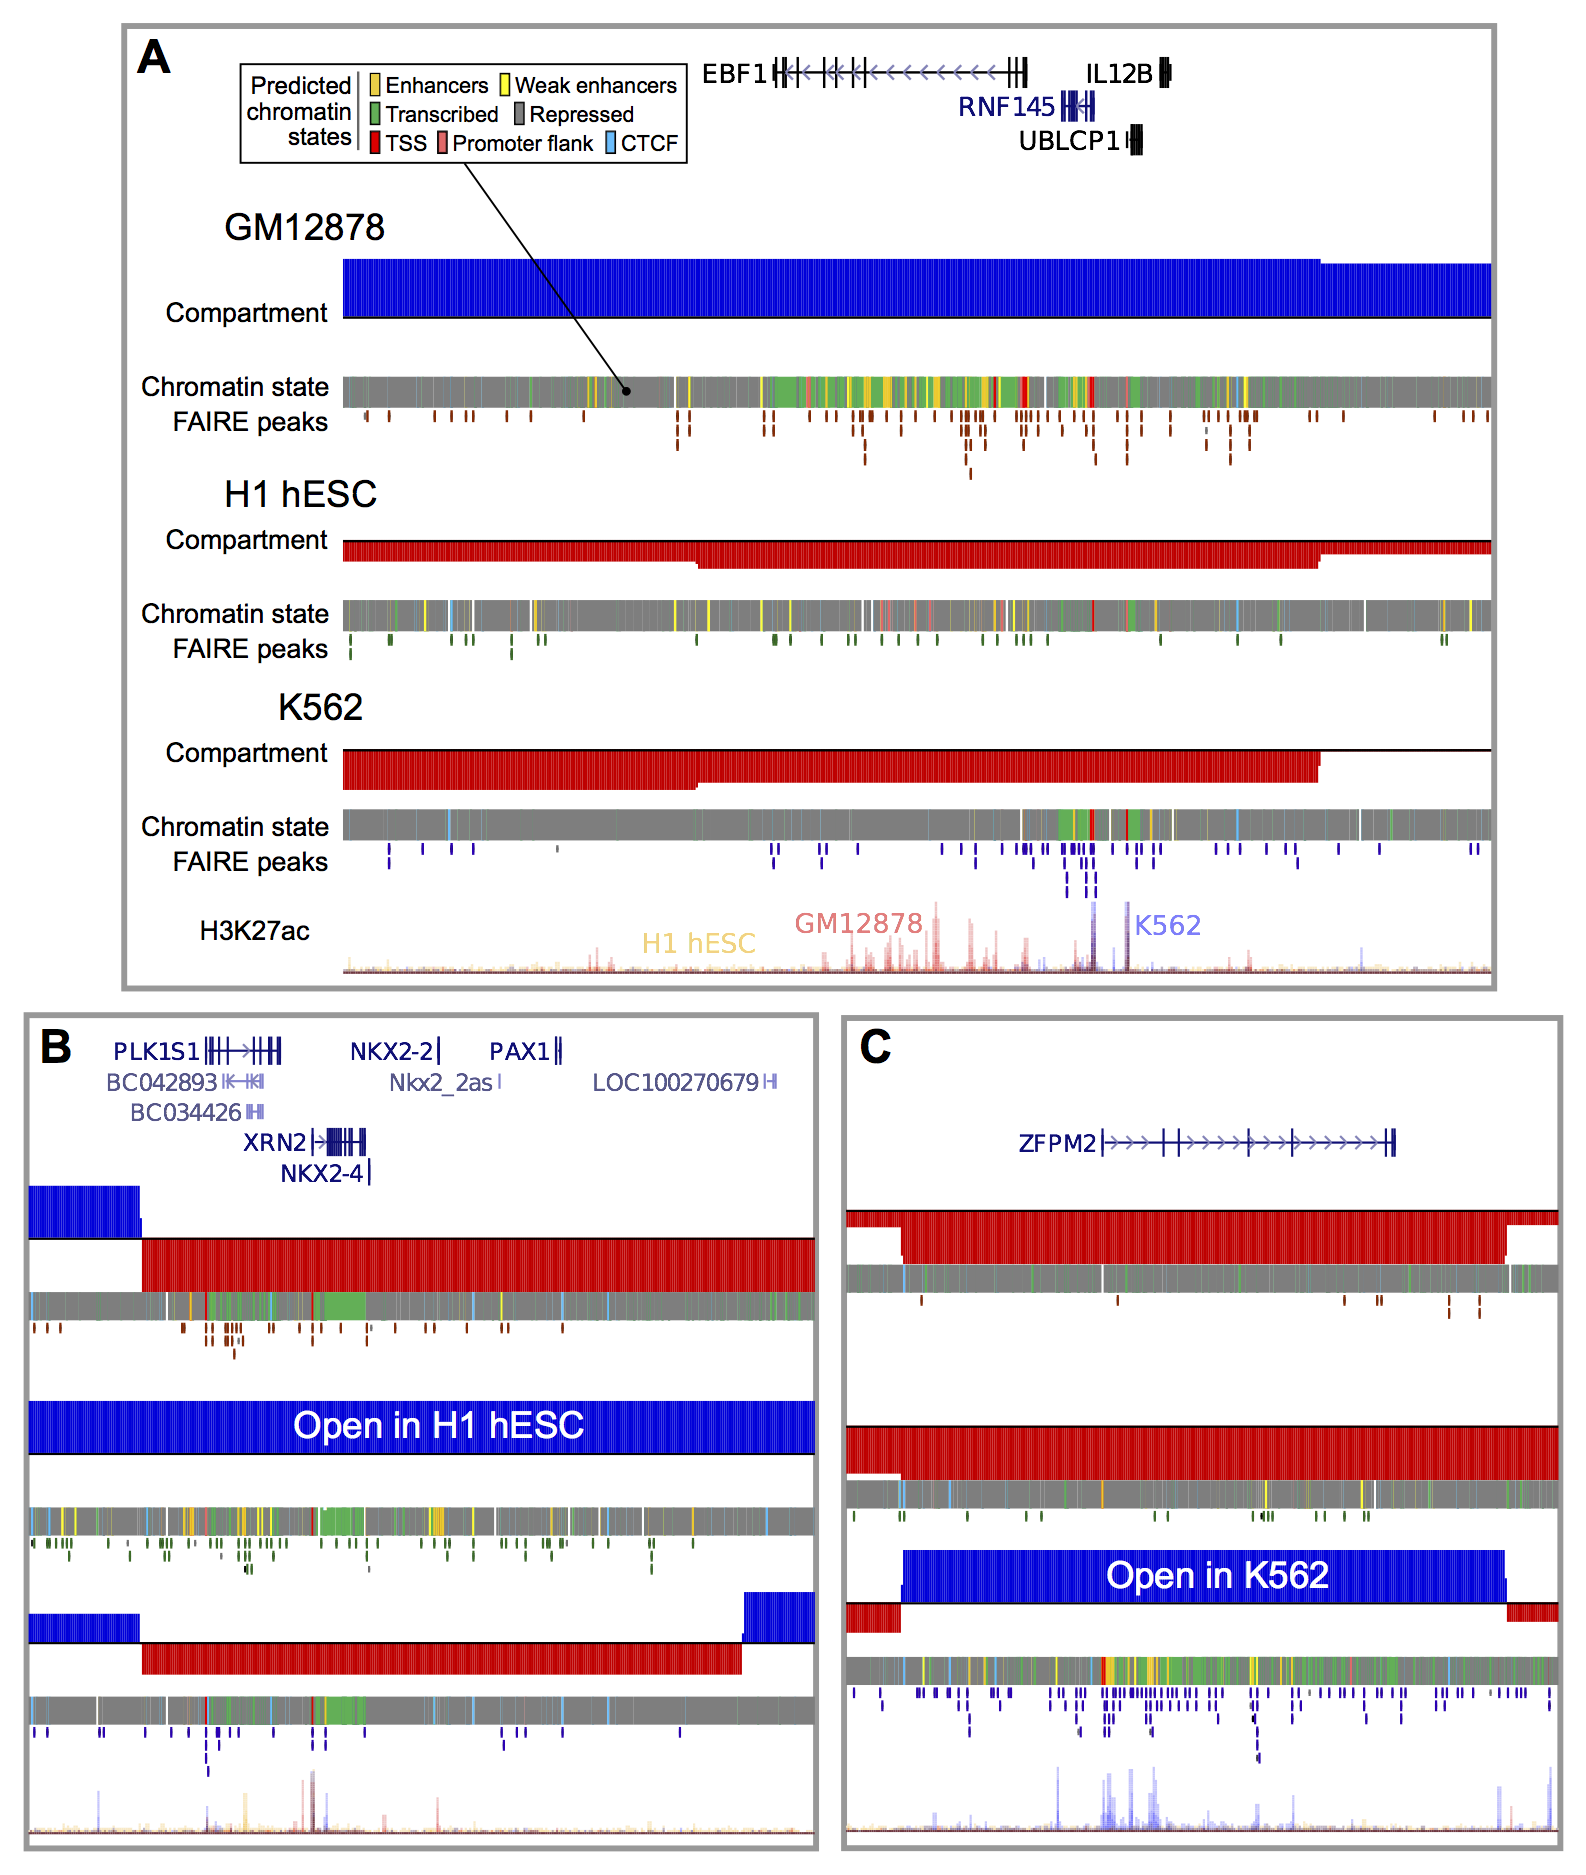
\includegraphics[width=.9\textwidth]{figs/examplervs.png}
\captionsetup{width=\textwidth} 
\caption{ {\bf Regions of variable structure alter their long-range contacts. }
Placeholder
}\label{fig:flippedegs}
\end{center} 
\end{figure} 

% fig 1.
\subsection{Chromatin state enrichment}


\subsection{Contact changes}

\begin{figure}
\begin{center} 
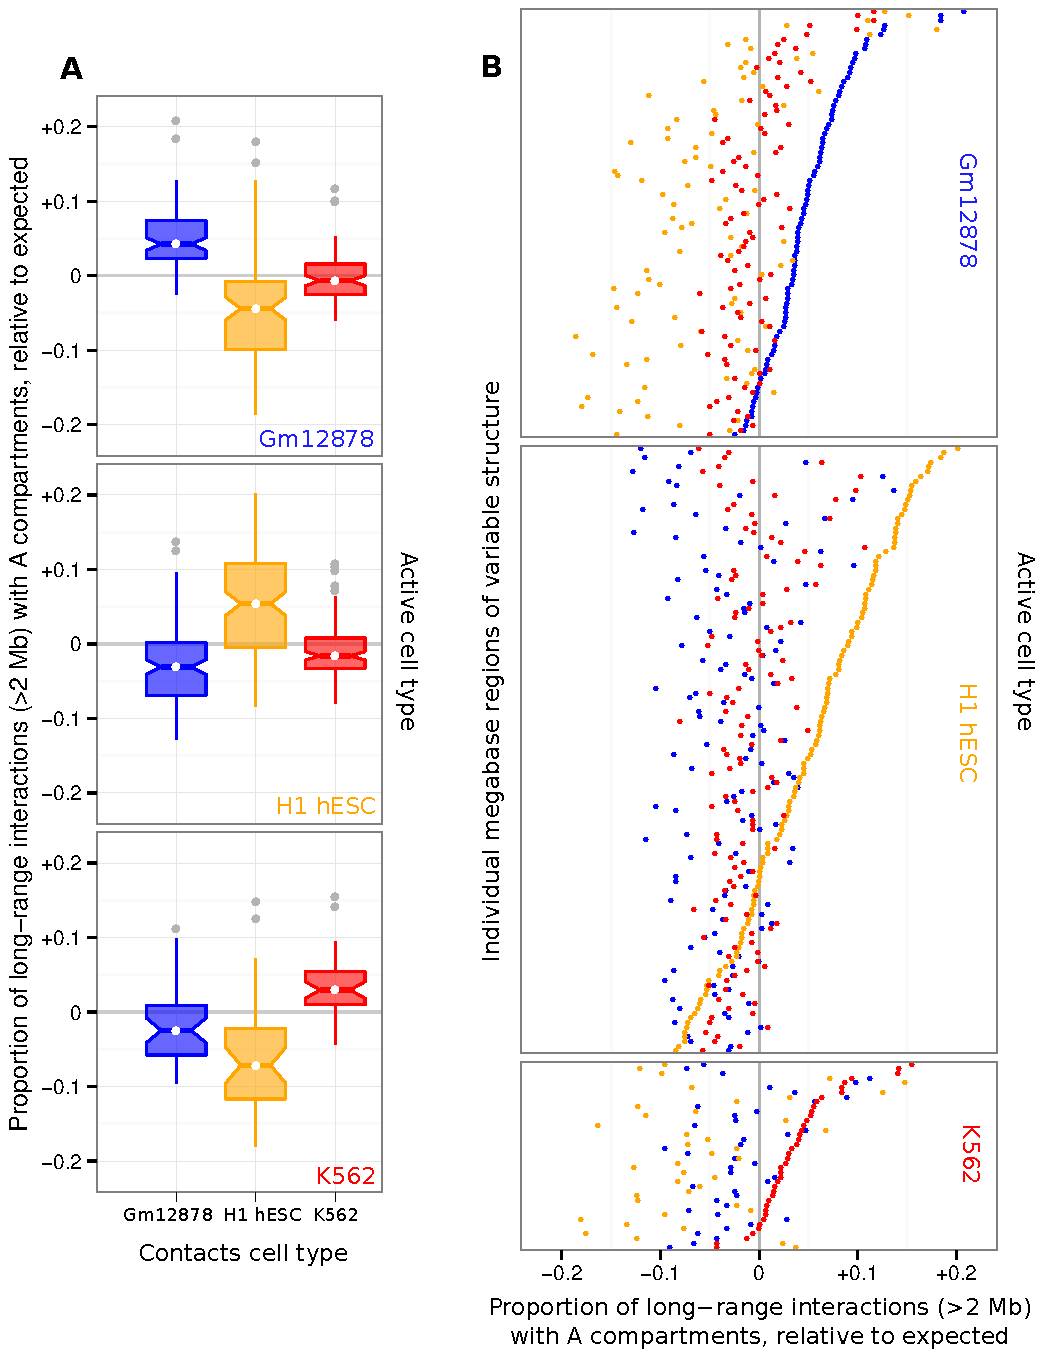
\includegraphics[width=.9\textwidth]{figs/longrange.pdf}
\captionsetup{width=\textwidth} 
\caption{ {\bf Regions of variable structure alter their long-range contacts. }
Placeholder
}\label{fig:longrange}
\end{center} 
\end{figure} 


\section{Nuclear positioning}

Chromosome positioning within the nucleus is known to reflect gene density, with the most gene-dense chromosomes occupying the centre of the nucleus in human cells.\cite{Bickmore2013} \citet{Kalhor2012} used a Hi-C variant to recreate probability density maps of chromosome positions which again reflected this feature of higher order chromatin organisation, and also reported active regions were more diffuse than inactive. A testable expectation with the eigenvector data used in this work is that active A compartments are enriched in the central nucleus of our human cell types, and B compartments are preferentially located in the nuclear periphery.

To test this, published data on chromosome positioning preference within
the nucleus was used to label chromosomes as ``central'' or 
or ``edge''.\cite{Boyle2001} Chromosomes whose DAPI hybridisation
signals were significantly enriched ($p\leq 2\times10^{-2}$) in the inner nuclear shell, as
defined by \citet{Boyle2001}, made up the ``central''
group and included chromosomes 1, 16, 17, 19 and 22. Similarly the ``edge'' group
had enriched signals ($p\leq 5\times10^{-3}$) in the outer shell relative to the inner nuclear
shell and included chromosomes 2, 3, 4, 7, 8, 11, 13 and 18. The remaining
chromosomes showed no significant preference to either inner or
outer nuclear shells at $\alpha = 0.05$.\cite{Boyle2001} 

We found that positive eigenvectors (reflecting A compartments) did show a modest relative enrichment in centrally-positioned chromosomes relative to those located at the nuclear periphery (Fig. \ref{fig:nucpos}). The significance
of the difference in distribution of eigenvectors in the central
and edge of the nucleus was determined by a two-sided Kolmogorov-Smirnov (K-S)
test, with the null hypothesis that there is no difference between the empirical cumulative
density functions of the central chromosome eigenvectors ($F_{central}$)
and peripheral ($F_{edge}$). The difference was found to be statistically significant in each cell type ($H_0: F_{edge} = F_{central}$; GM12878: $D = 0.11$, $p < 6 \times 10^{-4}$; H1 hESC: $D = 0.12$, $p < 8 \times 10^{-8}$; K562: $D = 0.10$, $p < 5 \times 10^{-3}$)

\begin{figure}
\begin{center} 
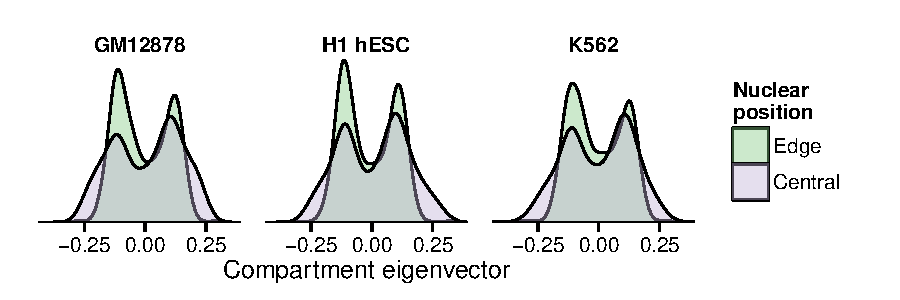
\includegraphics[width=\textwidth]{figs/nucpos.pdf}
\captionsetup{width=\textwidth} 
\caption{ {\bf Nuclear positioning of chromosomes relative to compartment eigenvectors. }
Kernel density estimates showing peripheral chromosomes have a greater proportion of B compartments (negative eigenvectors) relative to centrally-position chromosomes. Positioning data from \citet{Boyle2001} (Methods XX).
}\label{fig:nucpos}
\end{center} 
\end{figure} 


%\ifstandalone
\begin{small}
\bibliography{/Users/benmoore/Documents/library,/Users/benmoore/Documents/customrefs}
\end{small}
%\fi

\end{document}
